
\hypertarget{suxe9ance-3}{%
\chapter{Aḥmad Ibn Ḥanbal}\label{suxe9ance-3}}
\mn{Sequence 3 
Introduction à la théologie islamique classique}



Nous avons terminé notre séance sur le muʿtazilisme en évoquant la
tentative politique du calife d'imposer la doctrine de cette première
école de théologie islamique comme la doctrine officielle de l'État
abbasside. Cette tentative, appuyée sur la violence au besoin, s'est
soldée par un échec, car elle a rencontré une résistance trop
déterminée, incarnée par une classe sociale, celle des ulémas, des
hommes de religion, des traditionnistes. Si l'on a vu que leur approche
des questions théologiques pointait déjà, dans un refus de toute
théologie spéculative, cette épreuve va les obliger à opposer au
muʿtazilisme une doctrine plus construite et cohérente, et à théoriser
leur refus de cette manière de pratiquer la théologie. Cette doctrine
prendra bien vite le nom de son représentant le plus emblématique : le
traditionniste Aḥmad Ibn Ḥanbal (m. en 855).


\hypertarget{aux1e25mad-ibn-ux1e25anbal}{%
\section{Aḥmad Ibn Ḥanbal}\label{aux1e25mad-ibn-ux1e25anbal}}


L'imam Aḥmad Ibn Ḥanbal (que les auteurs sunnites désignent souvent sous
le seul nom de Aḥmad, pourtant si courant chez les Arabes) est un
traditionniste de Bagdad, de souche arabe, ayant notamment rassemblé une
importante collection de \emph{ḥadīṯ}-s prophétiques, le \emph{Musnad}.
Juriste connu comme rigoureux, il met au point une méthodologie
juridique qui se distingue de celles des \textbf{écoles de droit
religieux} qui commencent alors à se former.
\begin{Def}[Écoles de droit (maḏhab) ]
 Les ulémas qui ont cherché à expliciter la Loi divine, en se fondant sur le Coran et la Sunna, se sont progressivement organisés en écoles prenant le nom d’un maître ancien dont les méthodes ou les opinions servaient de source d’inspiration. C’est ainsi qu’ont progressivement émergé, en contexte sunnite, quatre principales écoles de droit musulman, qui existent jusqu’à nos jours : les malékites, les hanafites, les chaféites, les ḥanbalites. Ces écoles n’interprètent pas la Loi divine de la même façon, et diffèrent sur bien des points pratiques, mais elles se reconnaissent mutuellement comme légitimes. 
\end{Def}
Alors que ces dernières
accordent une place relativement importante au raisonnement du juriste,
en particulier le raisonnement par analogie, comme source du droit
islamique, Ibn Ḥanbal se montre méfiant à son égard ; s'il n'exclut pas
radicalement le raisonnement de la méthodologie juridique, il lui paraît
bien plus sûr, en cas de doute, de s'informer de l'attitude tenue en
pareil cas par le Prophète lui-même, au moyen des traditions
prophétiques, ces \emph{ḥadīṯ}-s dont il était précisément un
connaisseur. Après sa mort, des juristes se réclameront de sa méthode et
formeront une école de droit qui porte son nom, le ḥanbalisme, bien
qu'il n'ait pas eu l'objectif de devenir un chef d'école : au contraire,
dans son esprit, la Loi musulmane est à chercher dans ses sources, le
Coran et les \emph{ḥadīṯ}-s, et pas dans la pensée d'un savant tardif
comme lui !

\paragraph{Saint Patron confessant des traditionistes} Ibn Ḥanbal ne se serait sans doute pas aventuré dans les domaines de la
théologie proprement dite sans la contrainte imposée par le calife
al-Maʾmūn et ses successeurs de reconnaître le Coran comme « créé »,
comme nous l'avons vu dans la séquence précédente. La résistance d'Ibn
Ḥanbal aux pressions du calife, au point d'accepter d'être arrêté et
flagellé plutôt que de changer d'opinion, lui a donné une aura
extraordinaire, en particulier auprès des milieux les plus populaires de
la capitale de l'empire, Bagdad. On a pu parler de lui comme du « saint
patron des traditionnalistes » ! L'immense popularité de ce héros de la
résistance, affrontant les tortures du calife par amour de la vérité,
fera beaucoup dans l'échec de la \emph{miḥna}, cette « inquisition »
mise en place par les califes pour imposer par la force la doctrine des
muʿtazilites.

S'il est difficile de reconstituer avec certitude la pensée d'Ibn
Ḥanbal, une fois de plus faute de sources assurées, il semble qu'il ait
d'abord refusé de déclarer le Coran « créé », comme le réclamaient le
calife et les muʿtazilites, parce qu'il ne trouvait cette qualification
ni dans le Coran, ni dans les \emph{ḥadīṯ}-s, seuls fondements fiables
de notre connaissance théologique. Tous les raisonnements déployés par
ses adversaires ne pouvaient pas le convaincre, précisément parce qu'il
doutait des capacités de la raison humaine à parler de Dieu
adéquatement. Il semble au contraire que ces polémiques aient
progressivement durci
sa position. Dans une lettre (vraisemblablement authentique, pour une
fois !) au calife al- Mutawakkil (m. en 861), le calife même qui mettra
fin à la \emph{miḥna} et abandonnera le muʿtazilisme, Ibn Ḥanbal va plus
loin que ce prudent refus : il affirme cette fois positivement que le
Coran est incréé ; il l'est non seulement dans son contenu, ses idées,
mais encore dans ses mots même et jusque dans sa prononciation quand un
croyant le récite ; celui qui refuse de le dire, pour Ibn Ḥanbal, a
cessé d'être musulman. Cette évolution est significative : Ibn Ḥanbal,
en défendant leur foi traditionnelle contre les innovations
muʿtazilites, ont progressivement mis au point une doctrine capable de
la concurrencer.
\paragraph{Jésus créé par la parole éternelle}
Ibn Ḥanbal répond également à l'argument de Jahm Ibn Ṣafwān que nous
avons évoqué dans la première séquence, où le théologien affirmait que
le Coran est créé tout comme le Christ est une créature ; pour lui,
affirmer l'éternité du Coran, c'était donner des arguments aux chrétiens
qui soutiennent l'éternité du Christ. Ibn Ḥanbal juge l'argumentation
irrecevable : Jésus, explique-t-il, a été créé au moyen de la Parole de
Dieu, qui le précède parce qu'elle est précisément éternelle.


\hypertarget{une-approche-littuxe9raliste}{%
\section{Une approche littéraliste}\label{une-approche-littuxe9raliste}}


Beaucoup de traditionnistes proches d'Ibn Ḥanbal refusaient déjà de
faire du raisonnement une source du droit religieux : les commandements
de Dieu, estimaient-ils, ne s'inventent ni ne se déduisent ; ils se
reçoivent de la Révélation, c'est-à-dire le Coran ou la Sunna (la
tradition remontant au Prophète). 
\begin{Def}[sunnisme]
Du fait de leur attachement à cette
dernière, on commence à les appeler « les gens de la Tradition »
(\emph{ahl al-sunna}),
\end{Def}
ou « sunnites » \sn{C'est seulement plus tard que le mot « sunnisme » désignera la
confession majoritaire de l'islam, par distinction du chiisme en
particulier. À ce stade, le terme ne renvoie qu'à une école de théologie
et de droit, qui imposera peu à peu une partie de ses fondements comme
faisant partie de l'orthodoxie islamique.}.Pour Ibn Ḥanbal et ses
partisans, ce qui est vrai pour le droit islamique est encore plus vrai
pour la théologie, qui ne peut créer ses propres catégories, son propre
vocabulaire. Au contraire, estiment-ils, il faut parler de Dieu
seulement
\begin{quote}
    « comme il s'est décrit lui-même {[}dans le Coran{]}
et comme l'a décrit son Prophète {[}dans les \emph{ḥadīṯ}-s{]} »
(\emph{kamā waṣafa nafsahu wa-waṣafahu}
\emph{rasūluhu}).
\end{quote}

La prétention des muʿtazilites de « purifier » les textes sacrés en
neutralisant ce qui leur paraît incompatible avec la dignité ou la
transcendance de Dieu est jugée irrecevable par la plupart des savants
(\emph{ʿulamāʾ}, ou « ulémas ») issus de ce milieu : il s'agit pour eux
d'une forme de correction, au nom d'une raison toujours incertaine, de
la révélation divine elle-même ! De quel droit peut-on décider par
exemple que, là où Dieu ou le Prophète ont cru bon de parler des « mains
de Dieu », il s'agit en réalité de son action ou de ses grâces ? Si
c'était le cas, Dieu n'aurait-il pas pu le dire lui-même ? Comment
peut-on vider de son sens la promesse de Dieu qu'au paradis, nous le
verrons de nos yeux, en déclarant que Dieu n'ayant pas de corps, il est
par nature invisible à nos yeux et ne sera donc jamais vu ?

Cette lecture littéraliste du Coran et de la Sunna est qualifiée par les
muʿtazilites de \emph{tašbīh}, \sn{cf p. \pageref{def:Tasbih}} d'anthropomorphisme ; mais en retour, les
ḥanbalites accusent leurs adversaires de \emph{taʿṭīl} (littéralement,
le « dépouillement ») : ils ôtent à Dieu jusqu'aux attributs qu'il s'est
lui-même donné en se révélant, ce qui est bien plus grave. Quant à
l'identité des attributs et de l'Essence, ils apparaissent aux
ḥanbalites une inutile manière de refuser à Dieu les attributs les plus
évidents (la Science, la Puissance ou la Vie). 
\paragraph{Un succès populaire face à une théologie abstraite et élitiste} Le vif succès remporté
par les doctrines ḥanbalites dans les milieux populaires souligne
combien la théologie abstraite des muʿtazilites peinait à convaincre en
dehors de cercles intellectuels étroits : elle présentait un Dieu bien
peu compréhensible, très cérébral et conceptuel, offrant très peu de
prises à la piété ou à la dévotion. Les ḥanbalites, au contraire,
défendent le Dieu que chacun connaît, celui que décrit la lettre du
Coran, le Dieu du bon sens et de la foi de tous.

\paragraph{Adam à l'image de Dieu}Ibn Ḥanbal et ses premiers partisans étaient-ils anthropomorphistes ?
Leur effort de
compréhension littérale les amenait-il à concevoir un Dieu corporel
ressemblant à ses créatures ? C'est évidemment le reproche que ne
cessent de leur adresser leurs adversaires, mais cette question appelle
une réponse nuancée. Il semble qu'Ibn Ḥanbal ait refusé d'utiliser
le terme de « corps » à propos de Dieu, ce qui n'est pas surprenant : il
ne se trouve ni dans le Coran, ni dans les \emph{ḥadīṯ}-s. Mais devant
le \emph{ḥadīṯ} qui affirme, à l'instar de la Bible, que « Dieu a créé
Adam selon son image » (\emph{ḫalaqa Allāh Adam ʿalā ṣūratihi}), il
s'indigne que certains puissent comprendre « son image » comme l'image
d'Adam (l'arabe est aussi ambigu que le français sur ce point). Pour
lui, pas de doute : Adam a été créé à la ressemblance de Dieu ; ce qui
implique que Dieu a une image, une forme, qui ressemble à celle d'Adam.
Cela justifie du même mouvement l'usage, par les textes révélés, d'un
vocabulaire anthropomorphe. Mais Ibn Ḥanbal récuserait ce terme : ce
n'est pas Dieu, dirait-il, qui est anthropomorphe, mais l'homme qui est
théomorphe ; en d'autres termes, ce n'est pas Dieu qui ressemble à
l'homme, mais bien l'homme qui ressemble à Dieu !



  
  \subsection{Le \emph{bilā kayfa} : un argument fidéiste}
  



Comment toutefois accepter les multiples contradictions qui apparaissent
très vite quand on affirme à la fois que Dieu est transcendant, mais
qu'il a des mains ; qu'il est incorporel, mais qu'il se trouve en un
lieu (le septième ciel, comme l'affirme le Coran)\ldots{} Face à ces
difficultés, les ḥanbalites\sn{On ne trouve pas d'usage explicite de cet argument chez Ibn Ḥanbal
lui-même, mais il n'est pas douteux que
ses partisans en ont fait très tôt usage.} recourent à un argument emprunté au
traditionniste de Médine Mālik Ibn Anas (m. en 795), qui expliquait
ainsi le verset du Coran \emph{Le Miséricordieux est assis sur son
trône} (Coran 20, 5) : « Qu'Il soit assis est un fait connu, mais le
``comment'\,' est inconnu. Le croire est un devoir religieux, mais faire
des recherches à ce sujet est une \emph{innovation blâmable}. »
\begin{Def}[Innovation blamâble (bidʿa)]
 Les savants musulmans traditionnalistes, dans leur travail sur les ḥadīṯ-s en particulier, tendent à faire de l’action du Prophète la norme de l’action des musulmans. L’époque de Muḥammad étant considéré comme la meilleure, il ne saurait donc y avoir de progrès en matière religieuse. Toute nouveauté dans ce domaine, toute innovation qui s’écarte de la pratique du Prophète et de ses compagnons (les pieux ancêtres, ou salaf), sera donc vue avec suspicion par les traditionnalistes. L’accusation d’innovation (bidʿa) équivaut chez eux à une accusation d’hérésie. 
\end{Def}

L'argument consiste à distinguer le fait (Dieu a des mains, il est au
ciel) de son
« comment » (en arabe \emph{kayfa}), de la manière de l'expliquer. Le «
comment » des affirmations révélées à propos des attributs divins est
inconnu : on ignore comment Dieu a des mains, comment il peut être assis
sur son trône, comment il peut se mettre en colère. Le fait est vrai,
puisqu'il est révélé, mais il est « sans comment » (\emph{bilā kayfa}).
La transcendance de Dieu est ainsi respectée : on ne prétend pas tout
connaître de Dieu, encore moins tout en comprendre ; mais cela ne veut
pas dire, comme dans l'argumentation obscure des muʿtazilites, qu'on ne
peut rien connaître de Dieu, sinon qu'il est. Le Coran et les
\emph{ḥadīṯ}-s affirment à son sujet de nombreux éléments qu'un croyant
doit tenir pour vrai, sauf à mettre la parole de Dieu en doute. Mais
comment sont-ils vrais ? « Dieu est le plus savant, répond le bon
croyant : c'est Dieu qui le sait. »

Cet argument du « sans comment », ou \emph{bilā kayfa}, correspond assez
exactement à ce que la philosophie des sciences appelle le fidéisme,
l'attitude qui place la croyance religieuse sur un plan où les arguments
rationnels ne peuvent l'atteindre ni remettre quelque point que ce soit
en question.
\begin{Def}[Fidéisme] attitude religieuse qui discrédite d’avance le pouvoir de la raison dans la recherche d’une connaissance assurée, au profit de la seule foi. Elle estime que les vérités religieuses doivent être crues, mais qu’elles sont par essence incompréhensibles à la raison humaine, et qu’il est en conséquence inutile de les discuter. 
\end{Def}
\paragraph{Une approche juridique de la théologie} Ibn Ḥanbal ne vient pas sans raison du monde du droit : l'approche qu'il
défend consiste en effet à intégrer la théologie dans le domaine du
droit. Les musulmans distinguent deux types de contenu dans les textes
révélés : 
\begin{Def}[al-amr]
il y a d'un côté tout ce qui relève du commandement
(\emph{al-amr}) -- les interdictions, les obligations, etc. -- qui sont
le domaine privilégié du droit religieux, et de l'autre côté des
informations (\emph{ḫabar}), comme par exemple les histoires des
prophètes.
\end{Def}  
Là où les muʿtazilites considéraient tout naturellement que
les attributs divins relevaient du \emph{ḫabar}, de l'information donnée
sur Dieu, les ḥanbalites répondent qu'elles relèvent au contraire du
\emph{amr}, du commandement : \textsc{quand il parle de lui dans le Coran, Dieu
ne révèle pas sa nature, forcément inconnaissable, mais il demande qu'on
le qualifie par ces attributs. }Ce changement est d'une grande
importance, car il justifie l'approche fidéiste, qui se fonde sur un
agnosticisme pieux : on ne peut pas connaître la nature de Dieu
(\emph{bilā kayfa}), mais on ne connaît que sa volonté. La nature de
Dieu est profondément inconnaissable, bien plus hors d'atteinte en
réalité que l'essence divine des muʿtazilites. Cet agnosticisme pieux
est une forme très profonde de respect de la transcendance divine, que
l'acceptation des attributs anthropomorphiques ne brise qu'en apparence.
Car si Ibn Ḥanbal affirme avec
persévérance que Dieu a des mains, qu'il se met en colère ou qu'il
ressemble à l'homme --- parce que la Révélation le dit ---, il ne
prétend pas savoir au juste ce que signifient ces affirmations. Il croit
seulement qu'elles sont vraies, et que Dieu lui ordonne de les tenir
pour telles, non de disserter longuement sur leur signification
nécessairement hors d'atteinte.

\mn{Une question aussi vis à vis du processus de révélation de la vérité par rapport aux jurys ou à la démocratie telle que nous l'entendons avec un processus de vérité émergeant lentement}

\paragraph{Une position inexpugnable mais faible par son refus de la confrontation} Cette position est à la fois inexpugnable par définition, puisqu'elle a
d'avance disqualifié toutes les objections qui peuvent lui être faites,
et relativement faible : il est difficile, dans une controverse, de
refuser purement et simplement d'argumenter. Ibn Ḥanbal lui-même, qui ne
refuse pas la raison en bloc mais seulement son usage comme source du
savoir théologique, ne s'y tiendra pas strictement, et se risquera plus
d'une fois à avancer des arguments à ses opposants. Il est à noter du
reste que le mouvement ḥanbalite ne se tiendra pas toujours à l'écart de
cette théologie spéculative qui semble si éloignée de ses fondements
propres ; par la suite, plusieurs de ses représentants s'y adonneront,
non sans habileté, mais aussi non sans provoquer des débats à
l'intérieur de l'école. 

Le ḥanbalisme présente la particularité, unique en islam, d'être à la
fois une école de droit (et même une des quatre écoles classiques qui,
depuis le moyen âge, se partagent le monopole du droit religieux dans le
monde sunnite) et une école de théologie. 

À l'époque classique, elle n'a
été dominante ni dans l'un ni dans l'autre domaine, mais contrairement à
beaucoup de mouvements éphémères, elle s'est toujours maintenue. Creuset
initial du sunnisme théologique --- qui va peu à peu se diversifier ---,
le ḥanbalisme a pour lui les inconvénients de l'intransigeance, qui
l'empêchent de convaincre une majorité, mais aussi ses avantages, à
commencer par la cohérence. C'est qu'il cherche à tenir jusqu'au bout
l'affirmation de la transcendance radicale de Dieu, au point de priver
de signification intelligible ces attributs divins dont il se fait
pourtant le héraut et le défenseur.

\paragraph{Ne pas projeter une vision rigoriste des mouvements ultérieurs sur l'origine} Son image de rigorisme et de traditionalisme ne doit pas être
caricaturée : elle a aussi donné naissance, comme nous le verrons plus
tard, à des théologiens de grande envergure ;
elle a été un terreau fertile pour l'ascétisme et une spiritualité très
vive. Mais notre vision contemporaine du ḥanbalisme est marquée par son
renouveau dans des courants modernes : le wahhabisme, né au XVIIIe
siècle en Arabie, et le salafisme, mouvement de réforme né au XIXe
siècle, vont l'un et l'autre s'en réclamer à leur manière. Mais ce
néo-ḥanbalisme, apparu dans un contexte bien différent du ḥanbalisme
classique, ne doit pas nous le faire oublier la complexité du mouvement
originel.


\hypertarget{lecture}{%
\section{Lecture}\label{lecture}}


\emph{Nous allons à présent lire un extrait d'un autre « Credo », une
profession de foi attribuée à Ibn Ḥanbal. Les chercheurs pensent
aujourd'hui que le texte n'est pas de la main du maître, mais de
disciples venant quelques décennies après lui. Mais contrairement au
texte muʿtazilite étudié la dernière fois, il n'est pas l'œuvre d'un
adversaire du mouvement !}

\emph{Je n'ai pas mentionné toutes les références coraniques ou
prophétiques qui émaillent le texte, car il y en aurait énormément ! Mais cela ne doit pas vous surprendre à
ce stade.}

\subsection{EXTRAIT D'UNE PROFESSION DE FOI ATTRIBUE A IBN ḤANBAL
(\emph{Ṭabaqāt al-ḥanābila}, pp. 28-29)}
\begin{quote}
    Dieu sait toute chose, et rien ne lui est caché. Il est sur son Trône
au-dessus du septième ciel. {[}\ldots{]} Si un
innovateur\sn{Pour l'auteur, le terme est extrêmement négatif : un innovateur est
quelqu'un qui ajoute quelque chose de nouveau à la révélation,
naturellement parfaite. Tout ajout ne peut être que négatif. Dans la
littérature ḥanbalite, « innovation » (\emph{bidʿa}) est un synonyme d'«
hérésie ».} ou un opposant essaie de prouver le
contraire en employant les mots de Dieu, comme « Nous sommes plus proche
de lui que sa veine jugulaire » (Q 50, 16) ou « Où que vous soyez, il
est avec vous » (Q 57, 4), ou encore « Il n'y a pas d'entretien à trois
où il ne soit le quatrième\ldots{} Il est avec eux là où ils se trouvent
» (Q 58, 7), ou d'autres passages ambigus du Coran, alors réponds-lui
que ce que le Coran exprime par là, c'est la connaissance de Dieu. Car
si Dieu est assis sur son Trône au-dessus du septième ciel, le plus
élevé, s'il est séparé de toute créature, il n'est pourtant pas de lieu
que sa connaissance n'atteigne.

\end{quote}
\begin{quote}
    
Dieu a un Trône, et ce Trône a des soutiens qui le portent. Dieu est sur
ce Trône, et il n'a pas de limite ; et Dieu est celui qui connaît le
mieux ses limites. Dieu entend, cela ne fait pas de doute, et il voit,
cela ne fait pas de doute. Il est savant, et non pas ignorant, généreux
et non avare, patient et non précipité, doué de mémoire et non oublieux,
éveillé et non endormi, proche et non négligent. Il se meut, il parle,
il observe ; il voit, il rit, il se réjouit ; il aime, il hait ; il
éprouve de l'aversion et du plaisir ; il est en colère et mécontent ; il
est miséricordieux et il pardonne ; il rend pauvre et riche ; il est
inaccessible. Il descend chaque nuit au premier ciel de la manière qu'il
veut. « Rien n'est semblable à lui ; il est celui qui entend et qui voit
» (Q 42, 11). Les cœurs de ses adorateurs sont entre deux doigts du
Miséricordieux : il les retourne comme il le veut. Il a créé Adam par sa
main,
à son image. Les cieux et la terre, au jour du Jugement, seront dans la paume de sa main. Il pose son pied en Enfer. […]
Le Coran est la Parole de Dieu, par laquelle il parle. Il n’est pas créé. Si quelqu’un pense qu’il a été créé, c’est un jahmite\sn{Un jahmite est, théoriquement du moins, un partisan du théologien Jahm
ibn Ṣafwān (m. en 746), dont nous avons parlé à la première séance (A,
3). Sous la plume d'auteurs ḥanbalites, le terme signifie tout
simplement
« hérétique ».}, un infidèle. Si quelqu’un pense que le Coran est la Parole de Dieu, mais suspend son jugement et ne dit pas qu’il est incréé, il est encore pire que le précédent. Si quelqu’un pense que notre prononciation ou notre récitation du Coran est créée, alors que le Coran est la Parole de Dieu, c’est un jahmite . Et quiconque ne déclare pas que tous ces gens sont des infidèles sont dans la même situation qu’eux.
\end{quote}




\paragraph{Localisation de Dieu} Le premier paragraphe affirme la localisation de Dieu : au septième
ciel, c'est-à-dire en son lieu le plus élevé, selon une cosmographie que
le Coran hérite du judaïsme de l'Antiquité tardive, qui y plaçait
également Dieu. Le texte fera plus tard allusion à un \emph{ḥadīṯ} du
Prophète qui affirme que, la nuit, Dieu descend au premier ciel, le plus
proche de la Terre, pour écouter la prière des croyants. 
\begin{figure}[h!]
    \centering
    \sidecaption{Almanach, Turquie, XVII. Ce document a été présenté debut 2022 lors de l'exposition \emph{Art de l'Islam} à Nancy. il vient de l'ancien couvent des Recollets et son interprétation inconnue. }
    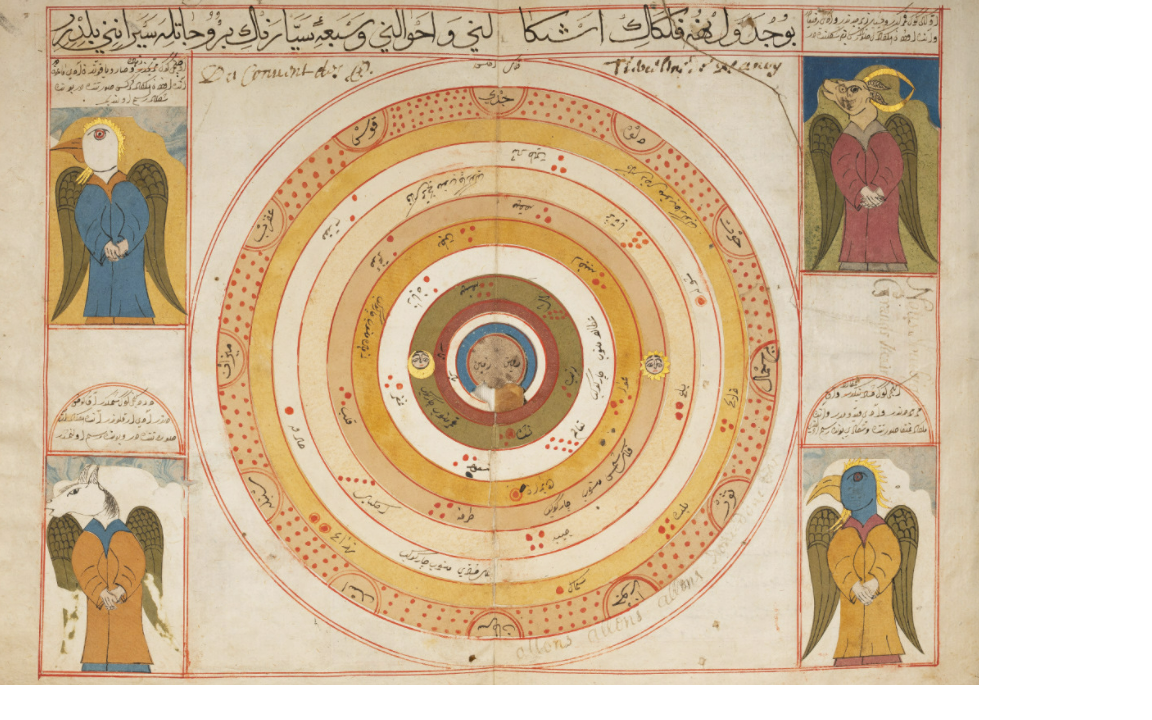
\includegraphics[width=\textwidth]{CoursCandiard/Image/AlmanachTurquie.png}
  
\end{figure}

\paragraph{Une interprétation} Les ḥanbalites
refusent de voir dans ce texte une simple image pieuse, destinée à
encourager les croyants à la dévotion nocturne : comme pour le septième
ciel, il s'agit du véritable lieu où Dieu se trouve à l'heure
mentionnée. À ce sujet, l'auteur ḥanbalite ne se contente pas de répéter
le texte coranique, mais fait droit à une objection : le Coran semble
placer Dieu en d'autres endroits que ce lointain septième ciel (et en
particulier sur terre, au milieu des hommes). La présentation de
contradictions entre des versets révélés est naturellement l'objection
la plus difficile à résoudre pour un littéraliste, qui est alors obligé
de s'écarter de sa propre règle : l'auteur donne, pour ces autres
versets, une interprétation qui n'est pas littérale (ces versets où Dieu
se dit présent auprès des hommes ne signifient pas une présence
physique, comme au sens littéral, mais sa connaissance de toute chose).
On remarque la limite inhérente à tout littéralisme : quand les textes
reconnus comme sacrés contiennent des contradictions internes, il est
impossible de
ne pas procéder à des formes d'interprétation du texte. Les théologiens
d'autres écoles ne manqueront pas, à toutes les époques, de relever les
nombreuses occurrences où le littéraliste Ibn Ḥanbal a lui-même
interprété les textes sacrés !

\paragraph{Le trône}Le deuxième paragraphe commence par une double affirmation paradoxale :
Dieu est sur un trône, que le texte décrit avec les mots du Coran ; et
Dieu n'a pas de limites. Comment peut-on tenir sur un trône, ou sur quoi
que ce soit, quand on est illimité ? C'est Dieu qui le sait, répond
l'auteur, faisant usage ici de la réponse \emph{bilā kayfa}, « sans
comment », que nous avons mentionnée.

Puis suit une énumération assez longue de qualificatifs attribués à
Dieu. Si notre texte précédent, le « credo » muʿtazilite, pratiquait lui
aussi les énumérations de ce genre, quelle différence sur le fond ! Car
l'auteur semble multiplier volontaire toutes les affirmations les plus
évidemment anthropomorphiques : Dieu se meut, il rit, il hait, il se
réjouit ou s'énerve\ldots{} Tous ces qualificatifs sont bien sûr ancrés,
soit dans le Coran, soit dans la Sunna. Le texte rappelle que, pour ces
textes sacrés, Dieu a des mains, qu'Adam est fait à son image, qu'il a
même un pied\ldots{} Cela n'empêche pas pour autant le texte de citer le
verset si cher aux muʿtazilites : « Rien n'est semblable à Lui ».
Comment cela est-il possible ? Le texte le rappelle à propos de la
descente de la nuit : il agit « de la manière qu'il veut ».

Dans le dernier paragraphe, enfin, le texte revient sur la question du
Coran créé, qui a provoqué la confrontation avec l'école muʿtazilite et
le pouvoir califal. L'auteur tient ici la position ḥanbalite la plus
radicale, qui affirme nettement, et sans aucune place possible pour le
doute et avec la plus grande intransigeance, que le Coran est incréé,
jusque dans sa prononciation : \textit{ce n'est pas un Coran céleste qui est
incréé, mais bien celui que le croyant récite le soir chez lui}. Ce
dernier point, qui peut nous paraître incroyablement excessif, mais il
souligne un point essentiel du ḥanbalisme primitif : le mouvement est
d'abord un mouvement de dévotion, porté par des personnes pieuses
occupées à apprendre par cœur le
Coran et les \emph{ḥadīṯ}-s, non dans une démarche intellectuelle, mais
pour se rapprocher de Dieu. Pour eux, la récitation du Coran est une
manière de rendre Dieu présent à leur adoration.

On notera que le texte ḥanbalite, bien moins abstrait que le « credo
muʿtazilite », est bien plus facile à lire. Ce n'est pas par hasard :
les deux groupes diffèrent par leur méthodologie, mais aussi par les
milieux auxquels ils s'adressent en priorité.

\section{Synthèse}

  1. Qu’est-ce qui semble inacceptable aux traditionnalistes dans l’approche théologique de l’école muʿtazilite ? 
  \begin{Synthesis}
  L'école mu'tazilite semble placer la raison devant le Coran et la Tradition, en décidant des \textit{attributs de Dieu} acceptables à la raison et ceux qui ne le sont pas. L'affirmation que le Coran est créé, n'apparaissant pas dans le Coran, elle n'est pas digne d'un article de Foi.
  \end{Synthesis}
  
  2.    Quels sont en revanche, pour leurs adversaires, les inconvénients du littéralisme ḥanbalite ? 
   \begin{Synthesis}
  Plusieurs critiques ont été opposées au littéralisme ḥanbalite :
  \begin{itemize}
      \item une approche fidéiste du bila kayfa, "comment" réservée à Dieu, certes inexpugnable mais une défense faible par son refus de toute discusion
      \item dans la pratique, certains passages du coran sont obscurs ou incohérents et nécessitent une interprétation, ce que Ibn Hanbal fera régulièrement.
      \item réduire la théologie au droit en considérant que les \textit{attributs de Dieu} sont de l'ordre du \emph{al-amr}, obligation, ne va pas naturellement de soi. C'est une interprétation en soi. 
      \item la position d'un Coran Incréé peut se comprendre par rapport à une position mu'tazilite d'un coran créé mais d'une certaine façon pourrait être aussi critiquée comme article de Foi d'innovation hasardeuse
  \end{itemize}
  \end{Synthesis}
  
  3. L’argument du bilā kayfa est-il une facilité pour éviter des obstacles rationnels trop nombreux, ou un véritable argument ? 
   \begin{Synthesis}
  Il découle d'un respect du texte et est un véritable argument. D'une certaine façon, il rejoint toutes les réactions fidéistes par rapport à des attaques hyper rationnelles (cf Renan au XIX) qui ne respectent pas le texte et la Foi des croyants.
  
  \end{Synthesis}


\section{Bibliographie}
\subsection{Instruments de travail}
On pourra consulter deux articles de l’Encyclopédie de l’islam (2e édition), tous deux écrits par l’islamologue français du XXe siècle H. Laoust : « Aḥmad b. Ḥanbal » (vol. 1, pp. 280-286) ; « Ḥanābila » (vol. 3-1, pp. 161-166). J. Hoover est l’auteur de l’article « Ḥanbalī Theology » du Oxford Handbook of Islamic Theology (sous la dir. de S. Schmidtke, 2016). Les premières pages (625-630) correspondent à la naissance du ḥanbalisme envisagé dans cette séquence.  

\subsection{Études}
 B. Abrahamov, Islamic Theology: Traditionalism and Rationalism, Édimbourg, Edinburgh University Press, 1998. 
 
 B. Abrahamov, « The "Bi-lā Kayfa" Doctrine and Its Foundations in Islamic Theology », in Arabica 42-3 (1995), pp. 365-379. 
 
 
 L. Holtzman, Anthropomorphism in Islam: The challenge of traditionalism (700-1350), Édimbourg, Edinburgh University Press, 2018. 
 
 G. Makdisi, L’islam hanbalisant, Paris, Geuthner, 1983. 